\chapter{Language Interpreter Design}
\section{Architecture}
the interpreter contains two part,the parser and the execution engine. the
parser will parse the source code into a parser tree,the execution engine will
then execute the code according to the parser tree.

\subsection{Parser}
the parser that the source code as input and generate a tree structure as
output.

\begin{figure}[h!]
  \centering
	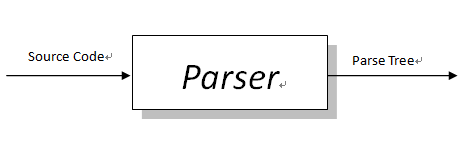
\includegraphics[width=0.80\textwidth]{pic/c4/parser.png}
	\caption{The Parser}
\end{figure}
the parser will contains different type of automata so that it could recognize different types of grammar.the grammar using to design the language
is content-free grammar.
the parser was build by combine simple and atomic parsers.The parser
can be view as a function that a parser is a function that takes a string of
characters as its argument, and returns a list of results.\cite{book}

\subsection{The Execution Engine}
The execution engine of the parser is basic on Haskell.the execution engine
will accept a parse tree and execute the command basic on this parse tree.
\begin{figure}[h!]
  \centering
	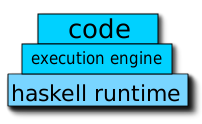
\includegraphics[width=0.40\textwidth]{pic/c4/structure.png}
	\caption{The Parser}
\end{figure}



\section{Imperative and Declarative language}
Declarative programming is a programming paradigm that expresses the logic of a computation without describing its control flow \cite{practical} while imperative programming paradigm is mainly about statement and manipulation of states.
\\ \\
In this project, the goal is to design an imperative language.Therefore,the design and interpretation of statement and assignment is the main focusing point in this project.
In addition,sub-function definition and function invocations support are also considered in this project to provide a certain level of abstraction.The table below has listed the fundamental statements.\\


\begin{tabular}{c|c}
\hline \textbf{Code} & \textbf{Description} \\
\hline  a = 1  &   assignment statement \\
\hline  a = fib () &  assignment statement with function invocation \\
\hline  while () {}&  while block statement\\
\hline if () {} &   if block statement \\
\hline for ( ; ; ) {} &  for block statement \\
\hline  fib(num1) &   function invocation  \\
\hline  break &   break loop control statement \\
\hline continue &   continue loop control statement \\
\hline 
\end{tabular} 

\section{Type System}
\subsection{Dynamic Typing and Static Typing}
A programming language is said to use static typing when type checking is performed during compile-time as opposed to run-time. 
For example , you have to specify the type explicitly and the compile will the the type correctness of a variable.A variable of a specified type can not assign to another value of other type.

\begin{tabular}{p{5cm}|p{5cm}}
\hline
Static Typing & Dynamic Typing \\
\hline
int a =1;\par \textbf{/*a is of type int */} \par int a="a string"; \par \textbf{ /* its not valid to assign a string to a variable that has type int */} & a=1; \par \textbf{/* does not need to specified a type for this variable */} \par a ="a string"; \par
\textbf{/* it valid to change the type of the variable */} \\ 
\hline
\end{tabular} \\\\
In my project, I used the dynamic typing scheme,which is ,does not need to specify any type of variable and able to assign any type of primitives to a variable.

\subsection{Strong Typing and Weak Typing}
a language is said to be strong typing is that it place restriction in operation where data type can not be intermix.


\begin{tabular}{p{6cm}|p{6cm}}
\hline Strong Typing & Weak Typing  \\ 
\hline a=123; \par 
\textbf{/* a is a number */} \par 
b="123" \par  
\textbf{/* b is a string */} \par 
c=a+b \textbf{/* return type error */}  &  
a = 123; \par 
b = "123"; \par
c = a+b; \par 
\textbf{/* either a will be convert to a string or b will be convert to a number */}

\\ 
\hline 
\end{tabular} 

In my project,I have implemented a weak typing system .I have design an statement call generic expression , which allow different kinds of value to intermix with each other. An expression like "12343" + 1232 -324 can be parse as follow syntax tree.




\section{Problem and resolution in writing BNF/EBNF rules}


For a parser , there are four operation it will do when encounters a terminal/non-terminal symbol.They are,
\begin{itemize}
\item Shift - push token onto stack
\item Reduce - remove handle from stack and push on corresponding nonterminal
\item Accept - recognize sentence when stack contains only the distinguished symbol and input is empty
\item Error - happens when none of the above is possible; means original input was not a sentence
\end{itemize}

Conflicts arise from ambiguities in the grammar when two or more operations and rules that apply to the same sequence of input.\cite{final}
\subsection{Shift//Reduce Problem}
A shift conflict occurs if there are two or more rules that
apply to the same sequence of input for the same operation reduce.  This usually indicates a serious
error in the grammar.

\subsection{Reduce//Reduce Problem}
A reduce/reduce conflict occurs if there are two or more rules that
apply to the same sequence of input for the same operation reduce.  This usually indicates a serious
error in the grammar.


\section{Syntax Design}

\subsection{The Main Structure}
A module is the minimum executable unit in \textbf{yun}.It is composed by one main function and serveral functions.The main function is a entry point,it may invoke other functions.

\begin{figure}[H]
  \centering
	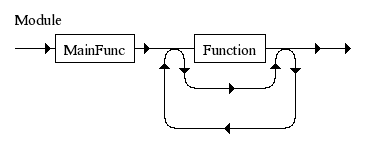
\includegraphics[width=0.90\textwidth]{pic/c4/module.png}
	\caption{Module Syntax Diagram}
\end{figure}

\begin{figure}[H]
  \centering
	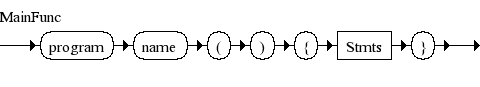
\includegraphics[width=0.90\textwidth]{pic/c4/main_function.png}
	\caption{Main Function Syntax Diagram}
\end{figure}

\begin{figure}[H]
  \centering
	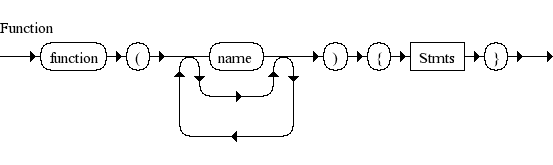
\includegraphics[width=1.00\textwidth]{pic/c4/function.png}
	\caption{Function Syntax Diagram}
\end{figure}


Possible program code may looks like follow,

\begin{lstlisting}[language=java]
program main ()
{
 	result = sum(1,2,3);
 	// more code
 	
}


function sum (var1,var2,var3)
{
	// body of the functions
}

// may be more functions
\end{lstlisting}


\subsection{Statements}
Statements  comprise the body of a function.A statement may be a assignment,break and continue sentence,return sentence.WhileBlocks ,IfBlocks,ForBlocks are all statements.What's more , WhilcBlock,IfBlock,ForBlock are recursively defined by statements as well.This allow nested for loop ,nested while loop and etc.

\begin{figure}[h!]
  \centering
	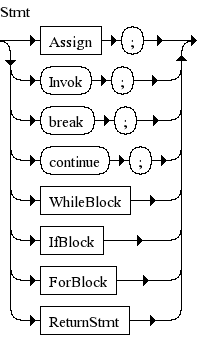
\includegraphics[width=0.45\textwidth]{pic/c4/stmt.png}
	\caption{Statement Syntax Diagram}
\end{figure}

The following code can be consider as a statement of the language
\begin{lstlisting}[language=java]
while ()
{
} /* the while statement */

if ()
{
}
else
{
} // the if else statement

for ( )
{
	for ()
	{
	}
} // nested for loop 


a = 1 ; // assignment statement, assign a value or and an expression to a variable

fib(5);  // function invocation statement


\end{lstlisting}

\subsubsection{Assignment}
There are three type of assignment in the language .They are ,
\begin{itemize}
\item Function invocation assignment.Assign the return result to a variable.
\item Generic expression assignment.Assign the result of an expression to a variable.
\item List assignment.Assign a list to a variable.
\end{itemize}
As \textbf{yun} is an imperative language,the right side of the assignment operator will be evaluation immediately. In other word,the language is strict.



\begin{figure}[h!]
  \centering
	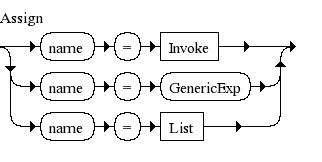
\includegraphics[width=0.65\textwidth]{pic/c4/assign.png}
	\caption{Assign Statement Syntax Diagram}
\end{figure}

\subsection{Generic Expression}
Generic expression represent the computation between primitives.As mention above, \textbf{yun} is  a weak typing and dynamic typing language,the generic expression accepts variant types of primitive and will do the conversion internally.


\begin{figure}[h!]
  \centering
	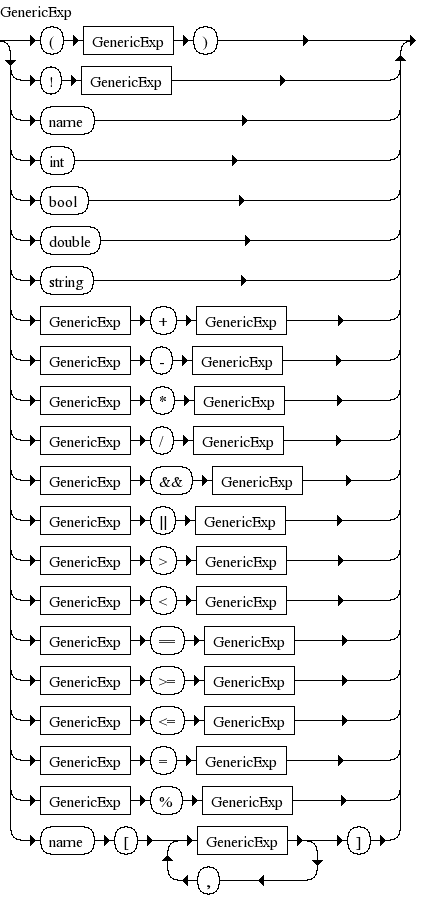
\includegraphics[width=0.65\textwidth]{pic/c4/generic_exp.png}
	\caption{Expression Syntax Diagram}
\end{figure}


Valid expression could be ,
\begin{lstlisting}[language=java]
"string"
1
-10 
1.1
True
False
True 
False // primitives 

1 + "a string"
1 * 2 + 1  
a && b
a || b
! a
a[2] //get the third element of a list
a[1,2]  // get the element in a multi dimension list

(a+b)+c // operation between variables
a[num] 
\end{lstlisting}


\subsubsection*{List}
The language support polymorphic list,the element of a list can be an expression or an list,thus the list support multi dimension list.If the element is an expression,the interpreter will evaluate it and store its result value in its internal format.

\begin{figure}[h!]
  \centering
	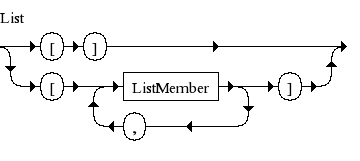
\includegraphics[width=0.69\textwidth]{pic/c4/list.png}
	\caption{Expression Syntax Diagram}
\end{figure}


\begin{figure}[H]
  \centering
	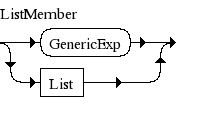
\includegraphics[width=0.45\textwidth]{pic/c4/list_member.png}
	\caption{List Member Syntax Diagram}
\end{figure}

Code Example

\begin{lstlisting}[language=java]
a = [1,2,3];
a = ["string",1,2,3];
a = [var1,var2,"other",var1+var2,True&&False]; 
a = [[1,2,3,4,5,6,7] , 1, 23.32, 5];
a = [1,2,3,4,5],[1,2,3,4],[3,45,43]]; // declare a multi dimension list

member = a[1] // get the second element of a list
\end{lstlisting}


\subsection{Code Block}
Code blocks including if block,while block and for block are statements.Code block may contains other statements which allow nested code block to be defined.



\begin{figure}[H]
  \centering
	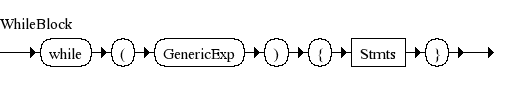
\includegraphics[width=0.95\textwidth]{pic/c4/while_block.png}
	\caption{While Block Syntax Diagram}
\end{figure}


\begin{figure}[H]
  \centering
	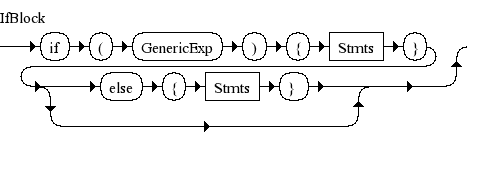
\includegraphics[width=0.95\textwidth]{pic/c4/if_block.png}
	\caption{If Block Syntax Diagram}
\end{figure}

\begin{figure}[H]
  \centering
	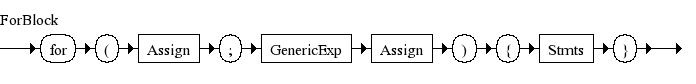
\includegraphics[width=0.95\textwidth]{pic/c4/for_block.png}
	\caption{for Block Syntax Diagram}
\end{figure}

Code Example,
\begin{lstlisting}[language=java]
if (a < 1){
	a = a+1;
	if ( a == 1){
		a = a-1;
	}	
}
else{
	a = a-1;
} // nested if loop


while (a<10){
	a= a+1;
} // while block


for (i =0;i<10;i=i+1){
	for (j=0;j<10;j=j+1){
		sum=j+i;
	}
}//nested for block

\end{lstlisting}
